\section{Application}
With the mathematical definition and deduction being discussed, we can now
look at the application of SVM in real life. Being a classification method,
SVM is widely used in many fields in order to distinguish data classes from
another. In this section, we will discuss five fields in which SVM is dominantly
utilized in: Face recognition, text classification,
bioinformatics and medical diagnosis, as well as handwriting recognition.

\subsection*{Face Recognition}
Face recognition is a biometric method that is widely used today in order
to identify a specific
person. It captures facial features such as eyes, chins, nose, et cetera and
uses the properties, for example, the distance or the angle between two parts, 
to distinguish a person from others. In reality, though, people do not always
look completely different from each other. The usage of SVM, 
in this case, strengthens the accuracy by its pattern recognition ability.

Since the basic theory of SVM is used to classify data, we
need to modify the learning algorithm in order to apply it to this pattern
recognition problem. The key here is to combine multiple SVM models in order
to construct a bottom-up binary tree. We compare each pair of nodes in the
tree and the winner of the comparison will be promoted to the upper level.
In the end, the unique class, which is the winner, will appear on the top of 
the tree. Given $C$ classes, this algorithm learns $C(C-1)/2$ SVM models at
the training phase and performs $C-1$ comparisons at the testing phase.

This algorithm is used on the Cambridge ORL face database for testing purposes, 
which contains 40 people with 10 face images per person.
The result shows that SVM performs better than other algorithms including
pseudo two-dimensional HMMs (Hidden Markov Model) with a 5\% error rate 
and CNN (Convolutional Neural Network) with a 3.83\% error rate. SVM has
only classified 3.0\% of the images incorrectly. In another experiment,
this algorithm is used to compete against the eigenface method
with the nearest center classification (NCC), which has been long applied
in the face recognition field. Nevertheless, SVM still outperformed NCC,
having scored an 8.79\% minimum error rate in comparison to NCC's 15.14\%.
\cite{face-recognition}
\begin{figure}[h]%
    \begin{center}%
        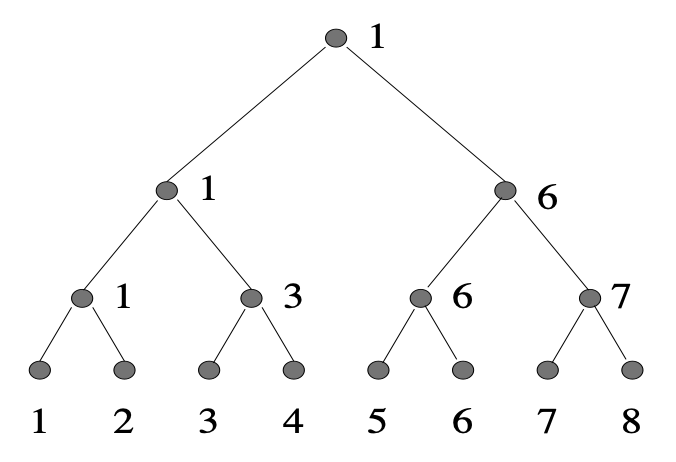
\includegraphics[scale=0.2]{Binary_Tree.png}%
        \caption{The binary tree structure for 8 classes face recognition.
        The numbers 1-8 encode the classes. 
        Each class is first compared to the nearby node,
        and the winner is promoted to the upper level.
        After $\log_2(8) = 3$ comparisons,
        the unique class number appears 
        on the top of the tree.
         \cite{face-recognition}}\label{fig:}%
    \end{center}%
\end{figure}

\subsection*{Text Classification}
Dealing with text data has long been a challenge in the machine learning
field, and this task is no exemption for SVM. In order to suit the algorithm
for text classification, we need to implement pool-based active learning
to the SVM model. The idea is that the learner has access to a pool of
unlabeled data and is allowed to request the label of some data points
in the pool.

Given a set of data points in a multidimensional space, we call the set
of hyperplanes to separate the data points in the version space. The goal of
the newly implemented algorithm is to reduce the version space as fast as
possible. Here, we introduce the idea of active learning, which consists of
a boolean classifier, a query strategy and a set of unlabeled data points.
In this case, we can choose the next query in a greedy way such that 
the version space is reduced as fast as possible. There are three ways
to instantiate this idea: 

\begin{itemize}
    \item \textbf{Simple Margin}: The algorithm picks the unlabeled instances
    in the pool whose hyperplane comes closest to the SVM unit vector, which is
    the center of the largest hypersphere that can fit inside the version space.
    \item \textbf{MinMax Margin}: For each unlabeled instance, compute the margins
    of the SVMs obtained when we label the instance as positive and negative
    respectively. Then, we choose the instance with the smallest margin.
    \item \textbf{Ratio Margin}: The algorithm works like MinMax margin, but uses
    the normalized margin instead of the absolute margin.
\end{itemize}

For inductive learning cases such as email filtering, a classifier is trained 
based on an SVM with a set of labeled data points.
For transductive learning cases such as relevance feedback, the classifier
learns an SVM with both labeled and unlabeled data points. In reality, it turns
out that combining MinMax margin and ratio margin methods delivers the best
result. \cite{text-classification}
\begin{figure}[h]%
    \begin{center}%
        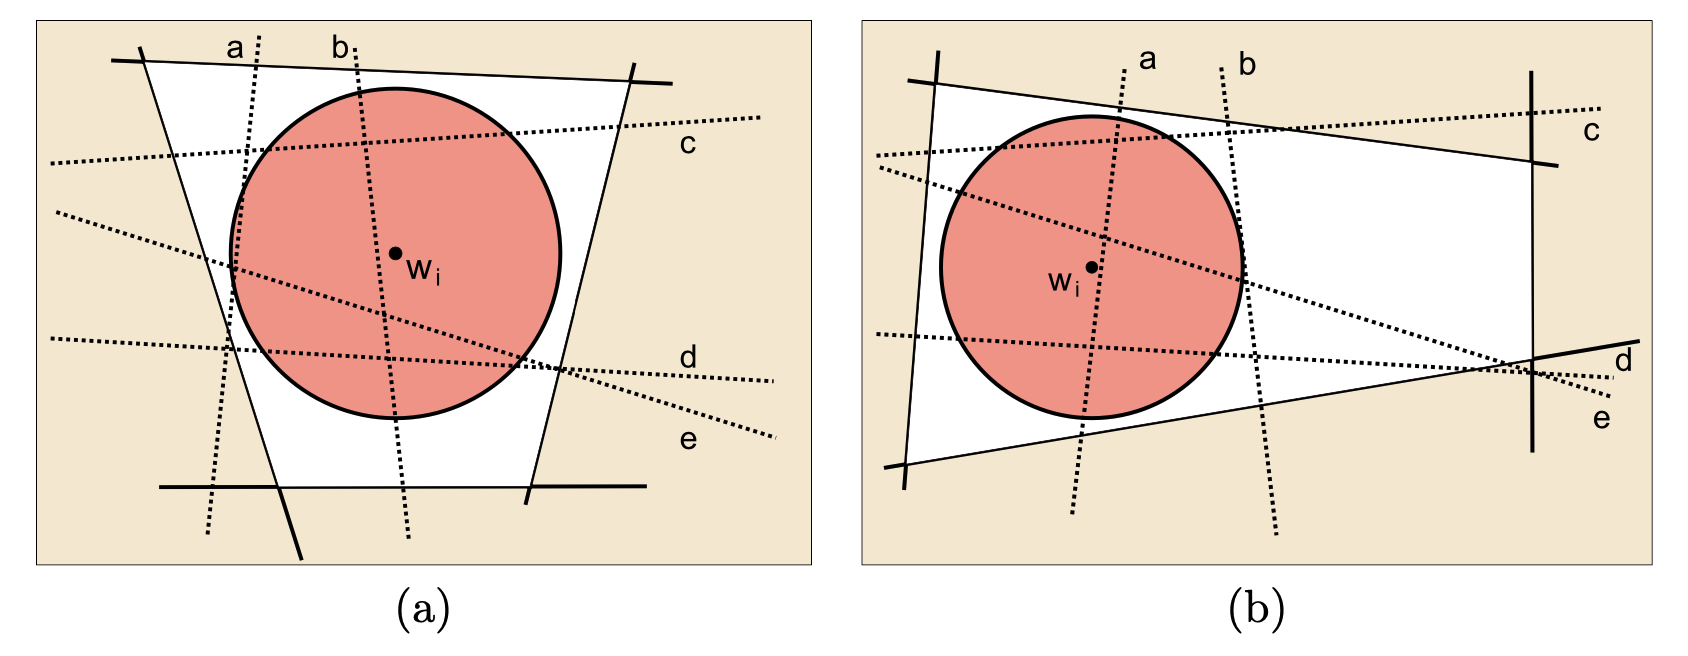
\includegraphics[scale=0.15]{Text_Classification.png}%
        \caption{
        A simple comparison of simple margin and MinMax margin.
        For this example, the simple margin will query \textbf{b},
        whereas the MinMax margin will query \textbf{a}.
        \cite{text-classification}}\label{fig:}%
    \end{center}%
\end{figure}


\subsection*{Bioinformatics}
In the bio-informatics field, two of the most common tasks are cancer
diagnosis and protein secondary structure prediction (PSSP). Since both of these
tasks are classification problems, SVM can be easily applied to them and is
capable of generating high accuracy results.

For cancer diagnosis, it is important to identify the types of cancer and the
responsive genes. However, all genes tend to have high dimensionality, while 
there are only a few samples available. For this problem, the research group
from Nanyang Technological University applied SVM with Welch's t-test.
The t-test shows the degree of differences between two groups of data points.
Here, we first apply the t-test to the data points based on which they are 
ranked. Afterwards, we select the top data points and apply SVM to them.
The result after applying this hybrid algorithm to several cancer datasets 
shows a very high accuracy score. For the SRBCT and the Lymphoma dataset, the
algorithm achieved a 100\% accuracy score. For the Leukemia dataset, the
algorithm only misclassified one instance out of 34 samples.

The PSSP problem is to predict the secondary structure of a protein. The
protein sequence is a linear array of amino acids, which is the basic unit
of a protein sequence. It consists of 3 consecutively ordered DNA bases (A, T, G, C). 
The secondary structure of the protein is formed between small segments of 
protein sequences with hydrogen bonds, which are mainly divided into 
three types: \emph{$\alpha$-helix}, \emph{$\beta$-sheet}, and \emph{coil}. 
In PSSP, we should classify the residues into these three types.
The algorithm consists of two phases: Sequence-Structure Prediction (Q2T) and
Structure-Structure Prediction (T2T). Q2T predicts the secondary structure
from the protein sequences, whereas T2T helps correct the errors
caused by Q2T. For Q2T, the SVM parameters alongside the window size are tuned
to train the model. For the window size of 13 and 15, the highest accuracy score
of 74.2\% is generated. T2T uses the output of Q2T as the input and corrects
the errors. The highest accuracy score achieved is 78.2\%.
\cite{bioinformatics}
\begin{figure}[h]%
    \begin{center}%
        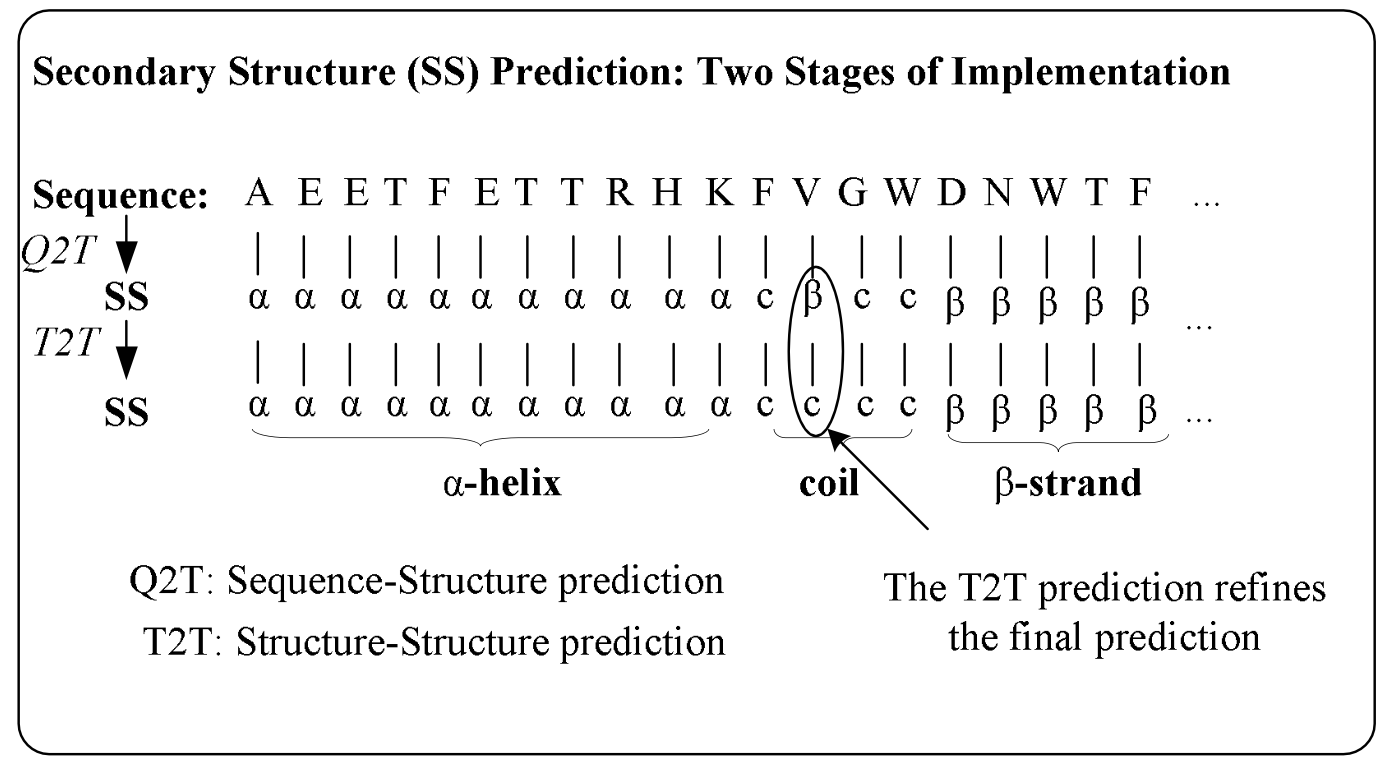
\includegraphics[scale=0.12]{PSSP.png}%
        \caption{Two phases of PSSP \cite{bioinformatics}}\label{fig:}%
    \end{center}%
\end{figure}

\subsection*{Handwriting Recognition}
The process of handwriting recognition consists of three phases:
pre-processing, feature extraction and classification. In the pre-processing
phase, the images undergo noise removal and binarization, skew detection
and correction, segmentation, as well as normalization and thinning. Then, 
the feature selection technique is implemented to determine the width/height
ratio, number of endpoints, number of cross points and number of branch
points. Finally, the SVM comes in to recognize the pattern. Like the usage of
SVM in face recognition, the SVM is used in a one-against-all fashion, so that
it can distinguish between different classes.

In an experiment conducted on a dataset of 10,000 handwritten isolated
Malayalam characters with 44 distinct characters, the dataset is divided
into 80\% training set and 20\% testing set and trained in five iterations
using cross validation. The SVM with polynomial kernel reports an average
accuracy of 90.83\%, whereas the SVM with radial basis function kernel
reports an average accuracy of 92.24\%, which is substantial subjected to 
this problem.
\cite{handwriting-recognition}
\begin{figure}[h]%
    \begin{center}%
        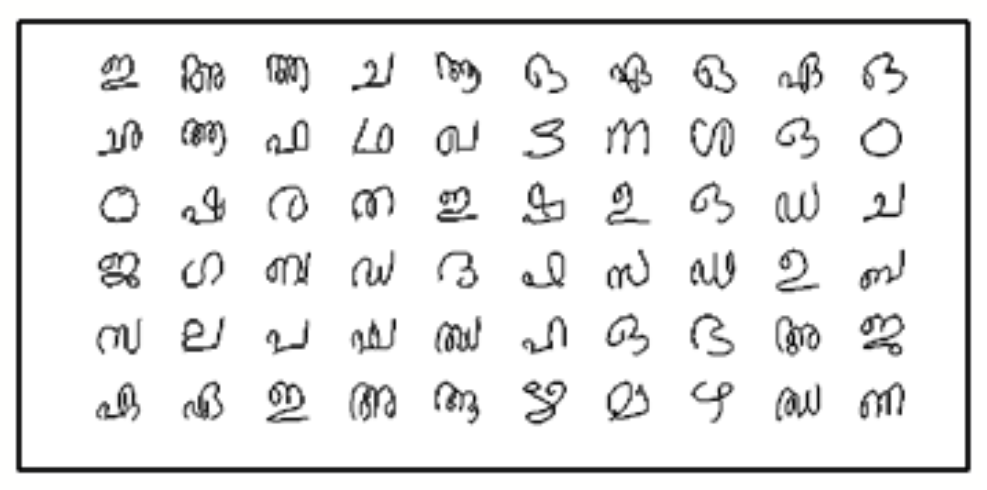
\includegraphics[scale=0.15]{Thinned_Handwriting.png}%
        \caption{Handwriting after binarization preprocessing \cite{handwriting-recognition}}\label{fig:}%
    \end{center}%
\end{figure}
